\documentclass[UTF8]{ctexart}

\usepackage{amsmath}
\usepackage{cases}
\usepackage{cite}
\usepackage{graphicx}
\usepackage[margin=1in]{geometry}
\usepackage{fancyhdr}
\usepackage{float}
\usepackage{listings}
\usepackage{ctex}
\usepackage{xcolor}
\usepackage{fontspec}
\usepackage{titling}
\pagestyle{fancy}
\fancyhf{}
\geometry{a4paper}

\lstset{ %代码块设置
    language = C,
    numbers=left,
    keywordstyle=\color{blue!70},
    commentstyle=\color{red!50!green!50!blue!50},
    frame=shadowbox,
    rulesepcolor=\color{red!20!green!20!blue!20},
    basicstyle=\ttfamily,
    showstringspaces=false
}
\lstset{language=C}

\title{Fashion-MNIST 图像分类实验报告}
\author{\LaTeX\ by\ xxx}
\date{\today}
\pagenumbering{arabic} %设置文章页码为阿拉伯数字

\begin{document}
\fancyhf{}
\fancyhead[L]{ %页眉左侧logo
    \begin{minipage}[c]{0.9\textwidth}
        
\includegraphics[height=10.5mm]{picture/logo.png}
    \end{minipage}
}
\fancyhead[C]{SSD 目标检测实验报告}
\fancyfoot[C]{\thepage}

\begin{titlepage}                                               %用于单人报告的封面 For single report 
    \centering
    
\includegraphics[width=0.65\textwidth]{picture/logo_text.png}   % 插入你的图片,调整文件名和路径 Insert your picture, adjust the file name and path
    \par\vspace{1.5cm}
    {\Huge \heiti SSD 目标检测实验报告 \par} % 标题 Title
    \vspace{1cm}
    {\Large \heiti 《计算机视觉》Assignment 2\par}              % 副标题 Subtitle
    \vspace{5cm}


    % 个人信息  Personal information
    \begin{center}
        {\Large                                                 % 这里的字号也可以用别的方式修改   The font size here can also be modified in other ways
        \makebox[4em][s]{\heiti 姓名}:\underline{\makebox[15em][c]{\heiti xxx}}\\
        \makebox[4em][s]{\heiti 学号}:\underline{\makebox[15em][c]{\heiti xxxxxxxxx}}\\
        \makebox[4em][s]{\heiti 班级}:\underline{\makebox[15em][c]{\heiti xxxxxxxxx}}\\
        \makebox[4em][s]{\heiti 学院}:\underline{\makebox[15em][c]{\heiti xxxxxxxxx}}\\
        }
    \end{center}

    \vfill
    \today % 日期
\end{titlepage}


\newpage

\tableofcontents  %自动根据下文创建目录


\newpage
\section{引言}

目标检测是计算机视觉领域的一项基础任务,其目标是同时实现物体的定位和分类。与仅需输出类别的图像分类任务不同,目标检测需要通过边界框(Bounding Box)准确标识出目标物体在图像中的位置,并给出相应的类别预测,这种"定位+分类"的双重任务使其在实际应用中具有重要价值。

目标检测模型主要分为两类:两阶段检测器和单阶段检测器。两阶段检测器如R-CNN系列(R-CNN、Fast R-CNN、Faster R-CNN)首先生成候选区域,然后对这些区域进行分类和边界框细化。这类方法精度较高但速度较慢。单阶段检测器如YOLO和SSD则直接在特征图上进行检测,省去了候选区域生成的步骤,因此具有更快的检测速度。

单发多框检测(SSD)是一种典型的单阶段检测器,其核心思想是利用多尺度特征图进行检测。具体来说,SSD在不同层次的特征图上设置不同大小和比例的锚框(Anchor Box),直接预测这些锚框的类别和位置偏移量。这种多尺度检测策略使得SSD能够有效处理不同尺寸的目标物体,同时保持较快的检测速度。

本实验将通过实现SSD的轻量级版本TinySSD,深入理解目标检测的基本原理和实现方法。

\section{实验目的}
本次实验主要围绕SSD目标检测模型展开,通过理论学习和实践操作,达到以下目的:
\begin{enumerate}
 \item \textbf{理解SSD的核心设计思想}:掌握单阶段检测器的基本原理,理解其相比两阶段检测器的优势。深入理解多尺度特征检测的概念,包括不同尺度特征图的作用。理解锚框(Anchor Box)机制在目标检测中的重要作用。掌握类别预测和边界框回归的基本原理。
    \item \textbf{掌握SSD的网络结构设计}:理解基础网络在特征提取中的作用。掌握多尺度特征块的设计原理和实现方法。理解类别预测层和边界框预测层的设计思路。掌握损失函数的设计原则,包括分类损失和定位损失的平衡。
    \item \textbf{实现简单的TinySSD模型}:手动实现TinySSD的核心组件,包括特征提取网络、多尺度特征块等。在一个较简单的数据集上训练和测试模型。通过实验验证模型的检测效果。
\end{enumerate}

通过完成上述目标,加深对目标检测任务的理解,掌握深度学习模型设计和实现的基本框架,为今后进一步学习更复杂的目标检测模型奠定基础。

\section{实验环境}
\subsection{硬件环境}
本实验使用个人笔记本电脑进行训练,i7 14650HX 处理器和 RTX 4060 Laptop 显卡的设备,CUDA版本为 12.6

\subsection{软件环境}
实验采用 Python 3.9,和 PyTorch 深度学习框架。自行实现了一些用于展示损失曲线的工具类。

\subsection{数据集}

受限于实验的硬件环境,本次实验使用了一个专门设计的香蕉检测小型数据集。这个数据集的特点如下:

\subsubsection{数据集构成}
\begin{itemize}
    \item 训练集:1000张图像
    \item 验证集:100张图像
    \item 图像尺寸:统一为256×256像素
    \item 每张图像包含一个香蕉目标
\end{itemize}
\subsubsection{数据集特点}
\begin{itemize}
    \item 图像中的香蕉具有不同的旋转角度、大小和位置
    \item 每张图像都配有标注信息,包括:目标类别(香蕉为唯一类别)和边界框坐标(左上角和右下角的x,y坐标,归一化到0~1范围)
    \item 香蕉图像被放置在各种不同的背景上,增加了检测任务的难度
\end{itemize}
\subsubsection{数据集格式}
\begin{itemize}
    \item 图像文件:以标准图像格式存储
    \item 标注文件:CSV格式,包含图像名称和对应的标注信息
    \item 标注信息格式:[类别, 左上x, 左上y, 右下x, 右下y]
\end{itemize}

这个数据集虽然规模较小,但包含了目标检测任务所需的基本元素,适合用于模型的原型验证和学习目标检测的基本概念。相比于COCO、Pascal VOC等大型数据集,这个简化的数据集可以帮助我们在个人电脑上更快地实现和测试TinySSD模型,同时理解目标检测的核心问题。

\section{TinySSD模型设计与实现}
\subsection{整体架构}

TinySSD作为SSD的轻量级实现,保留了SSD的核心设计思想,同时简化了网络结构。其整体架构如下:

\subsubsection{Backbone 网络结构}
TinySSD使用了一个简化的卷积神经网络作为 Backbone 网络,用于提取图像的初始特征:
\begin{enumerate}
    \item \textbf{输入层}:接收3通道、256$\times$256大小的图像
    \item \textbf{特征提取层}:
    \begin{itemize}
        \item 第一个卷积块:(3, 16, 3, 1) \hspace{0.5em} \# 输入通道,输出通道,卷积核大小,步幅
        \item 第二个卷积块:(16, 32, 3, 1)
        \item 最大池化层:(2, 2) \hspace{0.5em} \# 将特征图尺寸减半
    \end{itemize}
\end{enumerate}

\subsubsection{多尺度特征提取}
TinySSD采用多层特征图进行检测,这是实现多尺度目标检测的关键:
\begin{enumerate}
    \item \textbf{特征金字塔结构}:
    \begin{itemize}
        \item 第一级特征图:32$\times$32
        \item 第二级特征图:16$\times$16
        \item 第三级特征图:8$\times$8
        \item 第四级特征图:4$\times$4
    \end{itemize}
    
    \item \textbf{特征图转换}:
    \begin{itemize}
        \item 使用步幅为2的卷积层实现特征图的下采样
        \item 每个特征图都配备独立的类别预测层和边界框预测层
    \end{itemize}
\end{enumerate}

\subsubsection{锚框设计策略}
为了处理不同尺寸和形状的目标,TinySSD在每个特征图位置都设置了预定义的锚框:

\begin{enumerate}
    \item \textbf{锚框尺寸}:
    \begin{itemize}
        \item 较大特征图(32$\times$32):设置较小的锚框,用于检测小目标
        \item 较小特征图(4$\times$4):设置较大的锚框,用于检测大目标
    \end{itemize}
    
    \item \textbf{锚框配置}:
    \begin{itemize}
        \item 每个位置设置4个锚框
        \item 不同尺度比例:[0.75, 1, 2]
        \item 不同长宽比:[0.5, 1, 2]
    \end{itemize}
    
    \item \textbf{匹配策略}:
    \begin{itemize}
        \item 使用交并比(IoU)进行锚框与真实框的匹配
        \item IoU阈值设置为0.5
    \end{itemize}
\end{enumerate}
\subsection{核心组件分析}

\subsubsection{类别预测层实现与原理}
类别预测层负责预测每个锚框所包含目标的类别概率:
\begin{itemize}
    \item \textbf{结构设计}:
    \begin{itemize}
        \item 使用3$\times$3卷积层,输出通道数为 $num\_anchors \times (num\_classes + 1)$
        \item 每个锚框预测 $num\_classes + 1$ 个值,包含背景类
        \item 使用Softmax函数将输出转换为类别概率
    \end{itemize}
    \item \textbf{预测原理}:
    \begin{itemize}
        \item 对每个特征图位置的每个锚框进行类别预测
        \item 输出值最大的类别作为预测结果
    \end{itemize}
\end{itemize}

\subsubsection{边界框预测层设计}
边界框预测层用于调整锚框位置,以更好地匹配目标位置:
\begin{itemize}
    \item \textbf{预测内容}:
    \begin{itemize}
        \item 预测锚框的偏移量:中心点坐标偏移($\Delta x$, $\Delta y$)
        \item 预测尺寸缩放:宽度和高度的缩放因子($\Delta w$, $\Delta h$)
    \end{itemize}
    \item \textbf{实现方式}:
    \begin{itemize}
        \item 使用3$\times$3卷积层,输出通道数为 $num\_anchors \times 4$
        \item 对预测的偏移量进行边界框解码,得到最终的预测框
    \end{itemize}
\end{itemize}

\subsubsection{多尺度特征连接方式}
TinySSD采用自顶向下的特征融合策略:
\begin{itemize}
    \item \textbf{特征传递}:
    \begin{itemize}
        \item 高层特征通过上采样传递到低层
        \item 使用1$\times$1卷积层调整通道数
        \item 采用元素级加法进行特征融合
    \end{itemize}
    \item \textbf{特征重用}:
    \begin{itemize}
        \item 每个尺度的特征图都用于预测
        \item 不同尺度特征图负责不同大小目标的检测
    \end{itemize}
\end{itemize}

\subsubsection{损失函数设计}
模型采用多任务损失函数进行优化:
\begin{itemize}
    \item \textbf{分类损失}:
    \begin{itemize}
        \item 使用交叉熵损失函数
        \item 仅考虑正样本和部分负样本(硬负样本挖掘)
    \end{itemize}
    \item \textbf{定位损失}:
    \begin{itemize}
        \item 使用平滑L1损失函数
        \item 仅计算正样本的定位损失
    \end{itemize}
    \item \textbf{总损失}:
    \begin{equation}
        L = \frac{1}{N_{pos}}(L_{cls} + \alpha L_{loc})
    \end{equation}
    其中,$N_{pos}$为正样本数量,$\alpha$为平衡因子,设置为1.0
\end{itemize}

\section{实验结果分析}

\subsection{训练过程分析}
\begin{figure}[htbp]
    \centering
    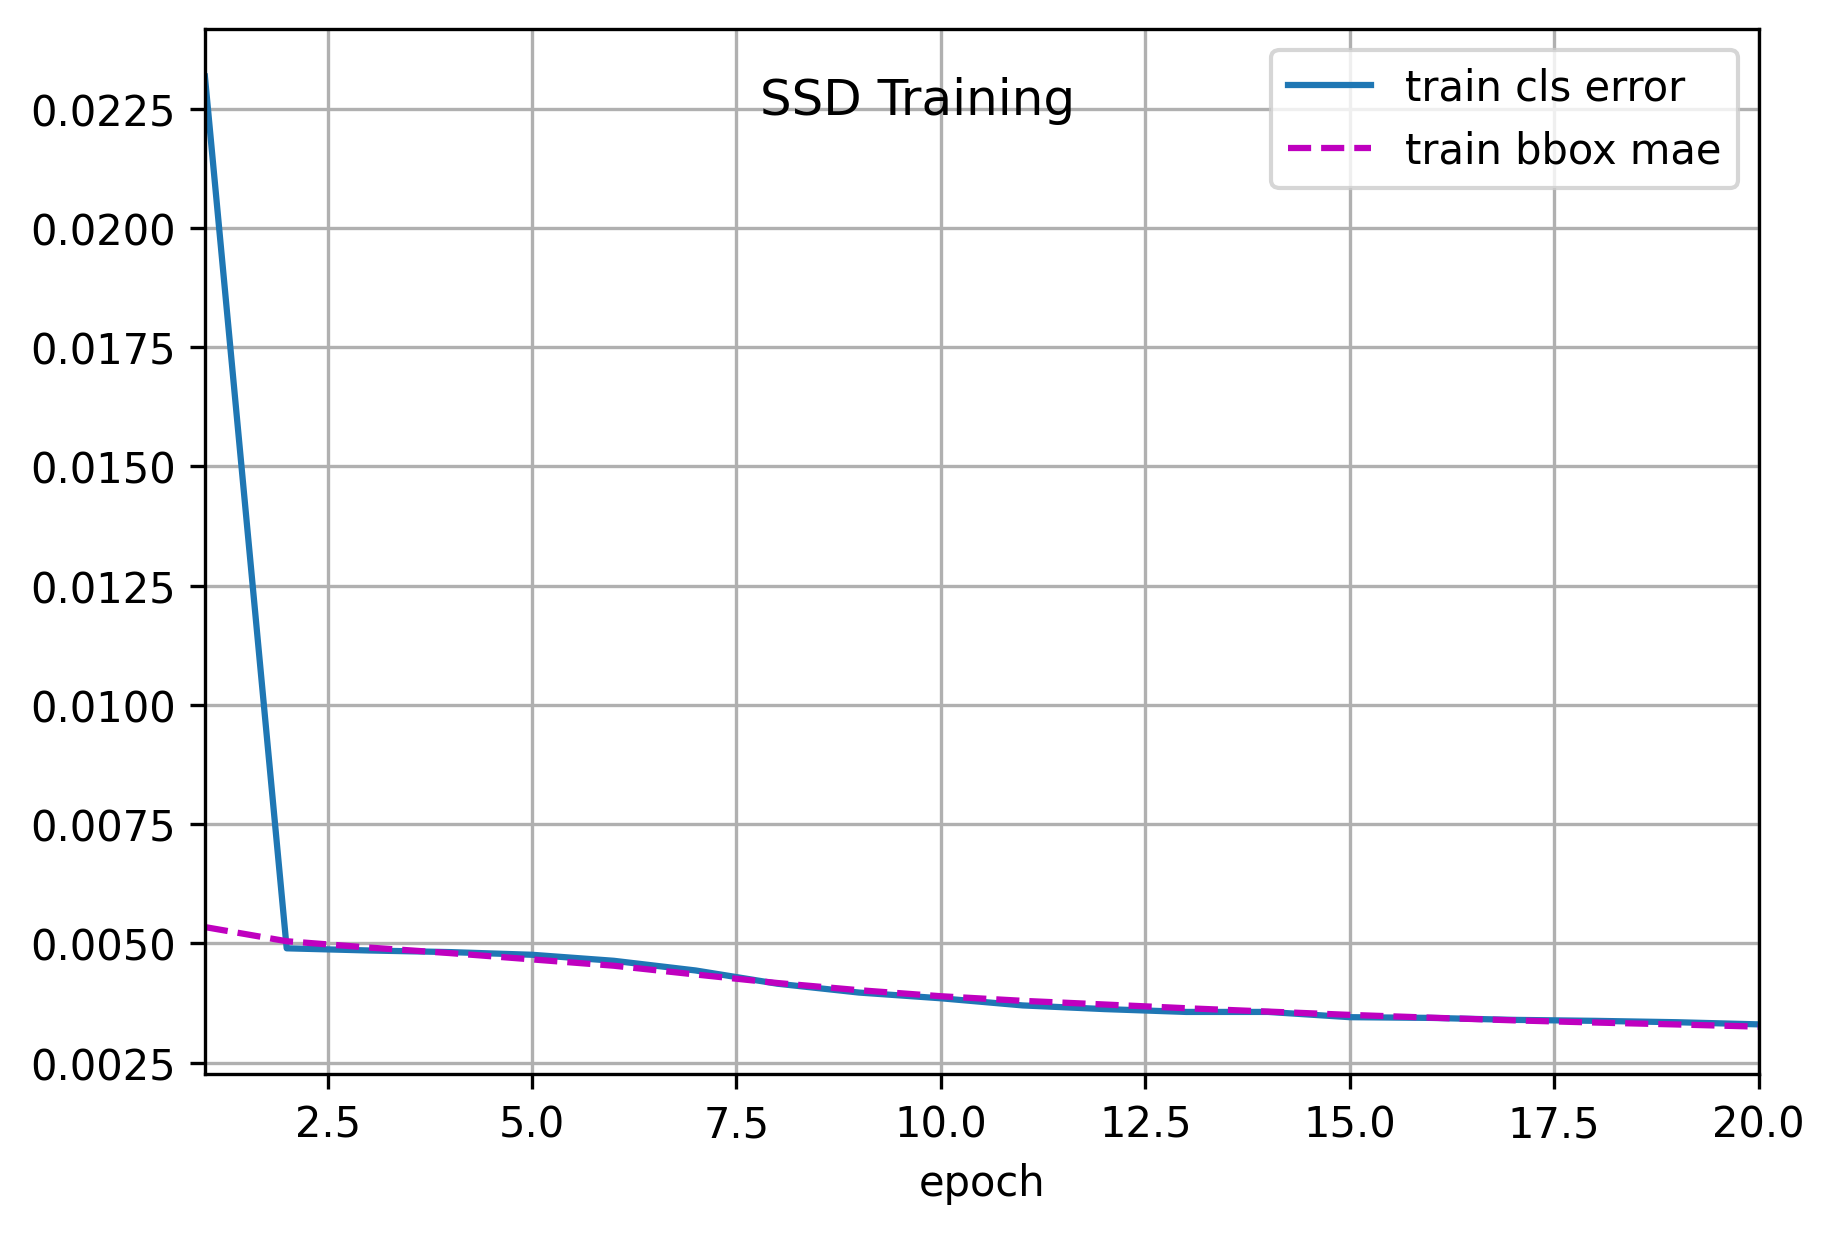
\includegraphics[width=0.8\textwidth]{picture/ssd_training_20241125_093259.png}
    \caption{TinySSD模型训练过程中的损失变化曲线}
    \label{fig:training_curve}
\end{figure}

\begin{itemize}
    \item \textbf{分类错误率变化}:
    \begin{itemize}
        \item 在训练初期(1-5轮)分类错误率快速下降,从0.0225降至约0.005
        \item 之后进入平稳期,错误率缓慢下降至0.003左右
        \item 最终趋于稳定,表明模型分类能力得到了良好训练
    \end{itemize}
    
    \item \textbf{边界框MAE变化}:
    \begin{itemize}
        \item 边界框平均绝对误差(MAE)整体呈下降趋势
        \item 初始阶段与分类错误率同步快速下降
        \item 在训练后期维持在较低水平,约0.003左右
    \end{itemize}
    
    \item \textbf{训练收敛性}:
    \begin{itemize}
        \item 模型在20轮训练后基本达到收敛
        \item 分类和定位损失都表现出良好的收敛特性
    \end{itemize}
\end{itemize}

\subsection{模型推理效果展示}

\begin{figure}[htbp]
    \centering
    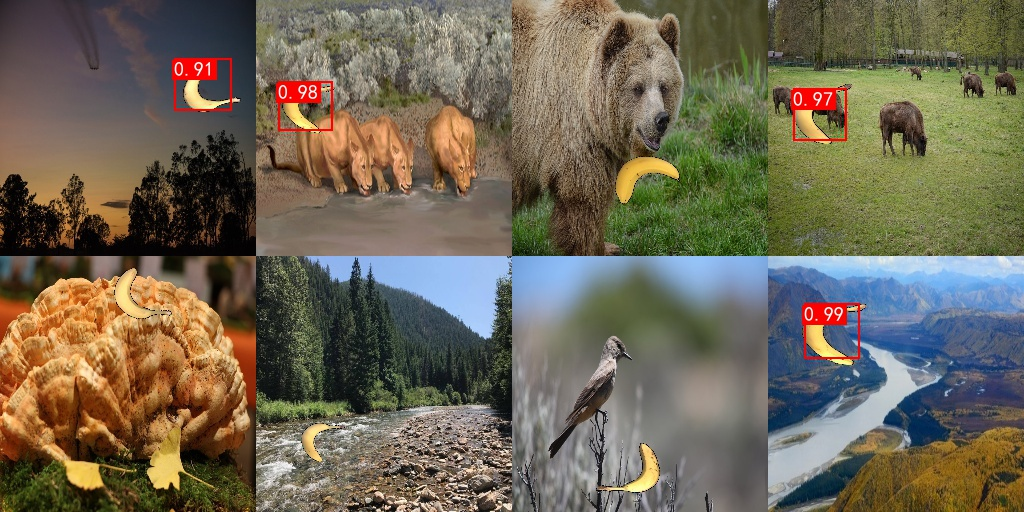
\includegraphics[width=0.9\textwidth]{picture/combined_predictions_1.jpg}
    \caption{TinySSD模型在不同场景下的推理结果}
    \label{fig:detection_results}
\end{figure}

从图\ref{fig:detection_results}的检测结果可以观察到以下特点:

\begin{itemize}
    \item \textbf{检测成功案例}:
    \begin{itemize}
        \item 模型在部分图像中成功检测出香蕉,置信度较高(0.91-0.99)
        \item 边界框的定位相对准确,能够较好地框住目标
    \end{itemize}
    
    \item \textbf{存在的问题}:
    \begin{itemize}
        \item 在复杂背景下(如河流、山脉场景)没能成功检测到香蕉的位置
    \end{itemize}
    
    \item \textbf{模型局限性分析}:
    \begin{itemize}
        \item 泛化能力不足,难以适应训练集之外的场景
        \item 对目标特征的学习过于简单,主要依赖形状特征
    \end{itemize}
\end{itemize}

\section{实验结论}

本次实验通过对 Fashion-MNIST 数据集的图像分类任务进行研究,对比了早期的 LeNet 网络与先进的 ResNet 模型,同时探究了超参数调优对模型性能的影响。
\begin{enumerate}
    \item 从模型性能方面来看,ResNet18 和 ResNet34 在测试准确率上总体优于 LeNet,这体现了先进的残差网络在特征学习能力上的优势。然而,LeNet 在合适的超参数下仍能取得不错的性能,说明对于特定的简单数据集,早期的经典模型也有其应用价值。
    \item 关于超参数调优,不同的学习率对各个模型的影响不同。较高的学习率(如 0.1)会导致模型训练不稳定,特别是对于 ResNet 系列模型而言,可能会使模型在更新参数时跳过最优解,从而难以收敛。而较低的学习率(如 0.01)虽然在训练过程中能使准确率较高,但会使模型的泛化性能略有下降,可能会陷入局部最优解,难以在测试集上取得良好的表现。这充分表明在模型训练过程中,合理选择超参数至关重要,它直接影响着模型的性能和收敛情况。对于此次任务下的模型,学习率为 0.05 时在训练和测试性能间取得了较好的平衡。
    \item 在计算效率方面,LeNet 由于结构简单,训练速度最快。随着 ResNet 模型层数的增加,训练速度逐渐降低。在实际应用中,需要根据具体的资源和性能需求来选择合适的模型。
    \item 通过本次实验,作为计算机视觉学习的起步,深入理解了深度网络的架构设计、图像分类的流程以及模型训练的关键环节。同时,也明确了不同模型在特定数据集下的适用性和局限性,为今后在计算机视觉领域的学习和实践提供了宝贵的经验。
    \item 对于未来的研究方向,可以进一步探索更多的超参数组合,尝试不同的优化器,以及实现模型集成等方法来进一步提升图像分类性能。同时,也可以将本次实验的方法应用到其他数据集上,进一步
\end{enumerate}
\section{总结与思考}

\subsection{TinySSD的特点}

\subsubsection{模型结构特点}
\begin{itemize}
    \item \textbf{轻量级设计}:
    \begin{itemize}
        \item 简化的基础网络结构,参数量较少
        \item 多尺度特征提取采用简单的特征金字塔结构
        \item 预测层设计简洁,计算效率高
    \end{itemize}
    
    \item \textbf{多尺度检测机制}:
    \begin{itemize}
        \item 采用四个不同尺度的特征图进行检测
        \item 特征图尺寸从32$\times$32递减至4$\times$4
        \item 不同尺度特征图负责不同大小目标的检测
    \end{itemize}
\end{itemize}

\subsubsection{优势与局限性}
\begin{itemize}
    \item \textbf{优势}:
    \begin{itemize}
        \item 计算效率高,适合资源受限场景
        \item 训练过程稳定,收敛性好
        \item 在简单场景下检测效果可靠
    \end{itemize}
    
    \item \textbf{局限性}:
    \begin{itemize}
        \item 特征提取能力有限,难以处理复杂场景
        \item 对目标形状和大小变化的适应性不足
    \end{itemize}
\end{itemize}

\subsubsection{适用场景分析}
\begin{itemize}
    \item \textbf{适合场景}:
    \begin{itemize}
        \item 单一目标、简单背景的检测任务
        \item 对实时性要求高的应用
        \item 资源受限的嵌入式设备
    \end{itemize}
    
    \item \textbf{不适合场景}:
    \begin{itemize}
        \item 复杂背景下的目标检测
        \item 多目标、多尺度的检测任务
        \item 要求高精度的专业应用
    \end{itemize}
\end{itemize}

\subsection{改进方向}

\subsubsection{可能的优化方向}
\begin{enumerate}
    \item \textbf{网络结构优化}:
    \begin{itemize}
        \item 引入更强大的特征提取骨干网络
        \item 改进特征融合机制,增强多尺度特征的表达能力
        \item 添加注意力机制,提升关键特征的提取能力
    \end{itemize}
    
    \item \textbf{训练策略改进}:
    \begin{itemize}
        \item 采用更先进的数据增强技术
        \item 改进损失函数设计,平衡定位和分类任务
        \item 引入在线难例挖掘(OHEM)等训练技巧
    \end{itemize}
    
    \item \textbf{后处理优化}:
    \begin{itemize}
        \item 改进非极大值抑制(NMS)策略
        \item 增加后处理规则,减少误检
        \item 引入置信度校准机制
    \end{itemize}
\end{enumerate}

\newpage
\section{附录:训练结果}
\subsection{TinySSD 检测效果示例}

\vspace*{\fill} % 上部填充

\begin{center}
\begin{minipage}{\textwidth}
\begin{figure}[H]
    \centering
    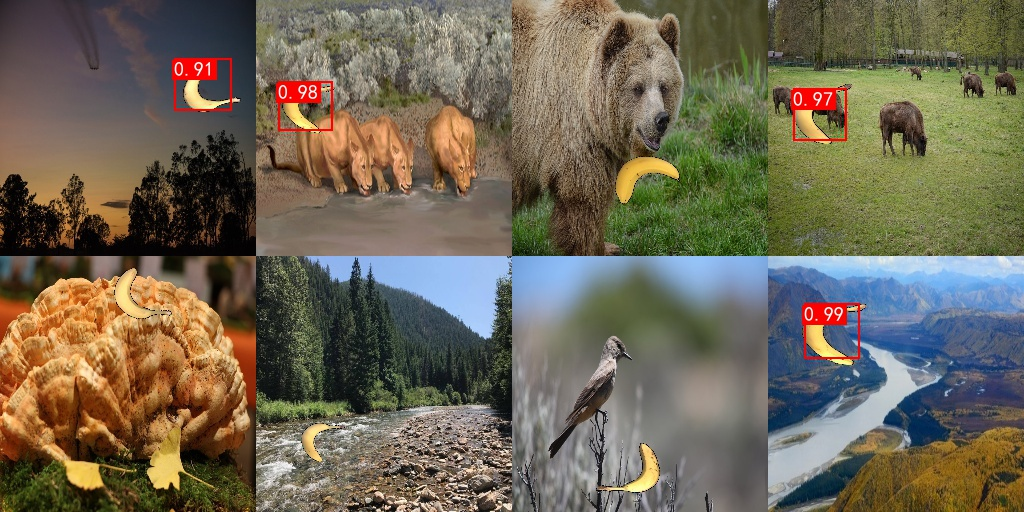
\includegraphics[width=0.8\textwidth]{picture/combined_predictions_1.jpg}
\end{figure}
\vfill

\begin{figure}[H]
    \centering
    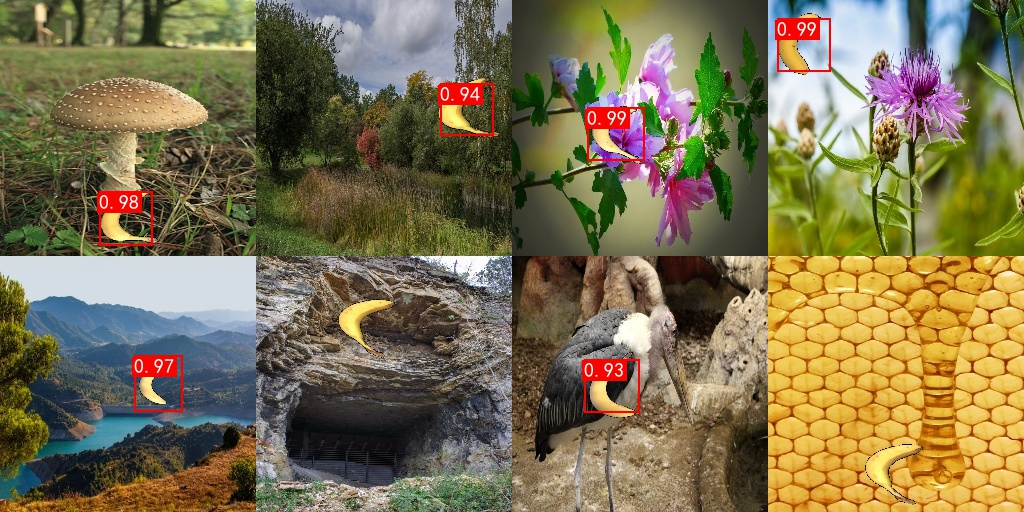
\includegraphics[width=0.8\textwidth]{picture/combined_predictions_2.jpg}
\end{figure}
\end{minipage}
\end{center}

\vspace*{\fill} % 下部填充

\newpage

\vspace*{\fill} % 上部填充

\begin{center}
\begin{minipage}{\textwidth}
\begin{figure}[H]
    \centering
    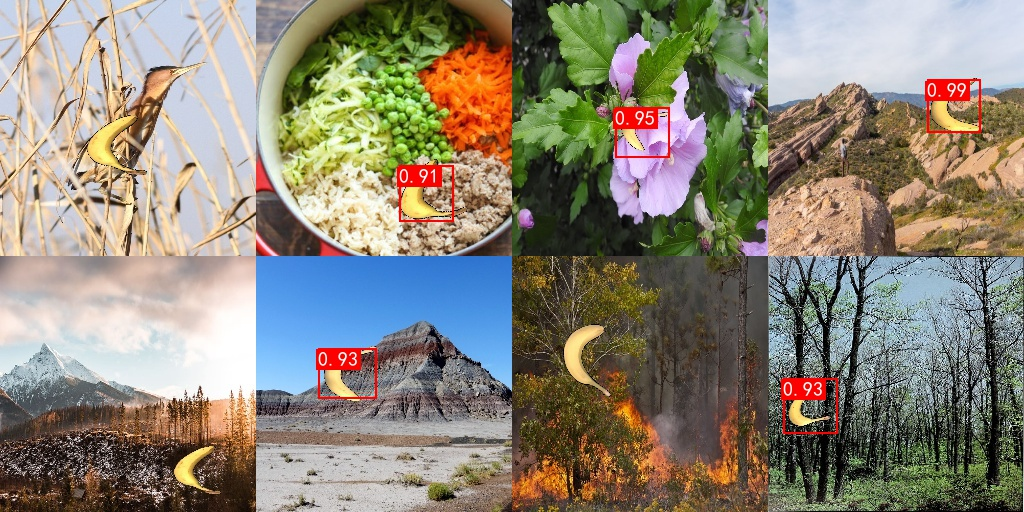
\includegraphics[width=0.8\textwidth]{picture/combined_predictions_3.jpg}
\end{figure}
\vfill

\begin{figure}[H]
    \centering
    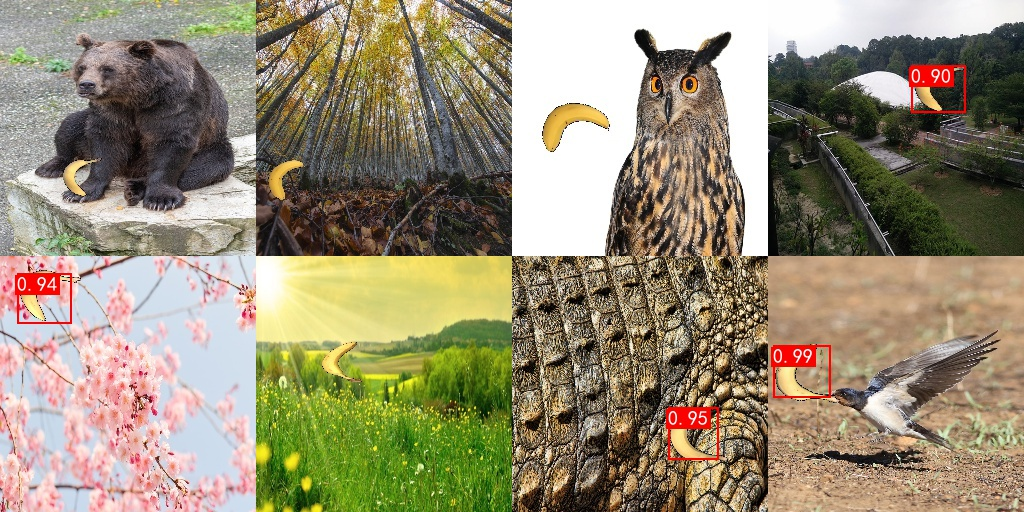
\includegraphics[width=0.8\textwidth]{picture/combined_predictions_4.jpg}
\end{figure}
\end{minipage}
\end{center}

\vspace*{\fill} % 下部填充


\end{document}